The implementation of the method has been designed to favor extensibility. The building blocks that compose the method, have been designed in an isolated fashion so that a practitioner may replace each one with one of his choice, without the method to collapse.

As mentioned in the previous chapter, as a general view the ROMC approach can be split into the training and the inference part; the training part contains all the steps until the computation of the proposal regions, while the inference part involves sampling, computing an expectation and evaluate the posterior. Apart from those main parts, the ROMC implementation provides some utilities for inspecting the training process, such as ploting the histogram of the distances $g_i(\theta_i^*)$ for choosing the threshold $\epsilon$ or visualizing the bounding box\footnote{if the parametric space is up to $2D$}. Finally, there are provide some functionalities for evaluating the obtain samples or the approximated posterior.

In the next three sections, we will provide an in-depth presentation of those ready-to-use functionalities. The main focus at this point is the illustration of the utilities that a practitioner may use out-of-the-box. For this reason we will use the a simple 1D example.

\subsubsection*{Simple 1D example}

For illustrating the implemented functionalities, we desing the following expample\footnote{In this example, the likelihood can be evaluated quite easily, hence it can be solved quite easily without a likelihood-free inference model. This is quite convenient at this point, since apart from illustrating the functionalities, we can quite easily validate the solutions obtained.}; the prior distribution is the uniform in the range $[-2.5, 2.5]$, i.e.\ $p(\theta) = \mathcal{U}(\theta;-2.5,2.5)$ and the generative model is the following,

\begin{gather} \label{eq:1D_example}
  p(y|\theta) = 
  \left\{
    \begin{array}{ll}
      \theta^4 + u & \mbox{if } \theta \in [-0.5, 0.5] \\
      |\theta| - c + u & \mbox{otherwise} 
    \end{array} \right.
\end{gather}

\noindent
where $u \sim \mathcal{N}(0,1)$. There is only one observation $y_0 = 0$.


The corresponding \textit{elfi} code for building the specific generative model is the following.

\begin{minted}
[framesep=2mm,
baselinestretch=1.2,
fontsize=\small,
]
{python}
  import scipy.stats as ss
  import elfi
  
  def simulator(t1, batch_size=1,random_state=None):
      if t1 < -0.5:
          y = ss.norm(loc=-t1-c, scale=1).rvs(random_state=random_state)
      elif t1 <= 0.5:
          y = ss.norm(loc=t1**4, scale=1).rvs(random_state=random_state)
      else:
          y = ss.norm(loc=t1-c, scale=1).rvs(random_state=random_state)
      return y

  y = 0
      
  # Elfi graph    
  t1 = elfi.Prior('uniform', -2.5, 5)
  sim = elfi.simulator(simulator, t1, observed=y)
  d = elfi.Distance('euclidean', sim)

  # Define ROMC inference method
  left_lim = np.array([-2.5])
  right_lim = np.array([2.5])
  romc = elfi.ROMC(d, left_lim=left_lim, right_lim=right_lim)
\end{minted}


\begin{figure}[!ht]
    \begin{center}
      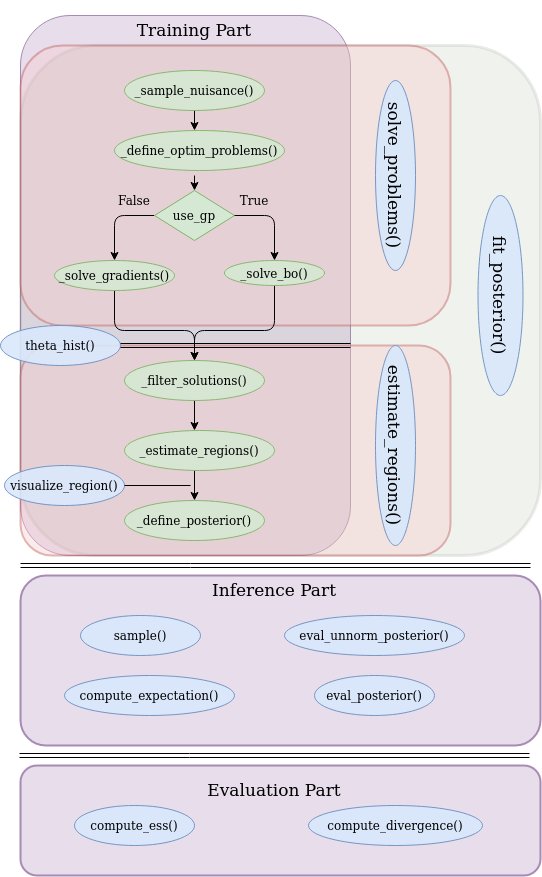
\includegraphics[width=0.75\textwidth]{./Thesis/graphs/ROMC.png}
    \end{center}
    \caption{Overview of the ROMC implementation. The training part follows a sequential pattern; the functions in the green ellipses must be called in a sequential fashion for completing the training part and define the posterior distribution. The functions in blue ellipses are the API calls that are called by the user.}
    \label{fig:elfi-model}
  \end{figure}

  